
\begin{frame}{Outline}

Outline for today:

\begin{itemize}
    \item Some examples of latent variable models
    \item A template: The Neyman-Scott ``paradox'' and marginalization
    \item Bayesian versus frequentist approaches to marginalization
    \item The classical EM algorithm
    \item The EM algorithm as variational inference
\end{itemize}

Next week, we will build on these ideas to present more general variational
inference.

\end{frame}

%%%%%%%%%%%%%%%%%%%%%%%%%%%%%%%%%%%%%%%%%%%%%%%%%%%%%%%%%%%
%%%%%%%%%%%%%%%%%%%%%%%%%%%%%%%%%%%%%%%%%%%%%%%%%%%%%%%%%%%
%%%%%%%%%%%%%%%%%%%%%%%%%%%%%%%%%%%%%%%%%%%%%%%%%%%%%%%%%%%


\begin{frame}{Latent variable models: Microcredit effectiveness}

\begin{columns}
    \begin{column}{0.5\textwidth}
Randomized controlled trials were run in seven different countries to measure
the effect of access to microcredit on business profits.
In each country, thousands of businesses were observed.  These businesses share
common, unobserved attributes of their particular country.
\citep{meager2020aggregating}

\vspace{1em}

The different levels of profit and microcredit effectiveness in each country are
latent variables.  We wish to infer the overall average effectiveness of
microcredit, which is common to all observations.

    \end{column}
    \begin{column}{0.4\textwidth}
        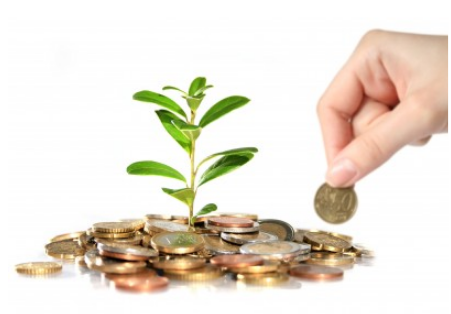
\includegraphics[width=1.0\textwidth]{static_images/microcredit.png}
    \end{column}
\end{columns}


\end{frame}


%%%%%%%%%%%%%%%%%%%%%%%%%%%%%%%%%%%%%%%%%%%%%%%%%%%%%%%%%%%
%%%%%%%%%%%%%%%%%%%%%%%%%%%%%%%%%%%%%%%%%%%%%%%%%%%%%%%%%%%
%%%%%%%%%%%%%%%%%%%%%%%%%%%%%%%%%%%%%%%%%%%%%%%%%%%%%%%%%%%


\begin{frame}{Latent variable models: Mouse geonmics}

\begin{columns}
    \begin{column}{0.5\textwidth}

A set of mice were infected with an influenza virus, and the expression level
for a large number of genes were measured over time.  We wish to cluster
together genes that have similarly shaped expression time series.
\citep{Luan:2003:clustering}

\vspace{1em}

The cluster identities (archetypical time series of expression levels)
are common to all observations.  Which cluster a particular gene belongs to
is a latent variable.


    \end{column}
    \begin{column}{0.4\textwidth}
        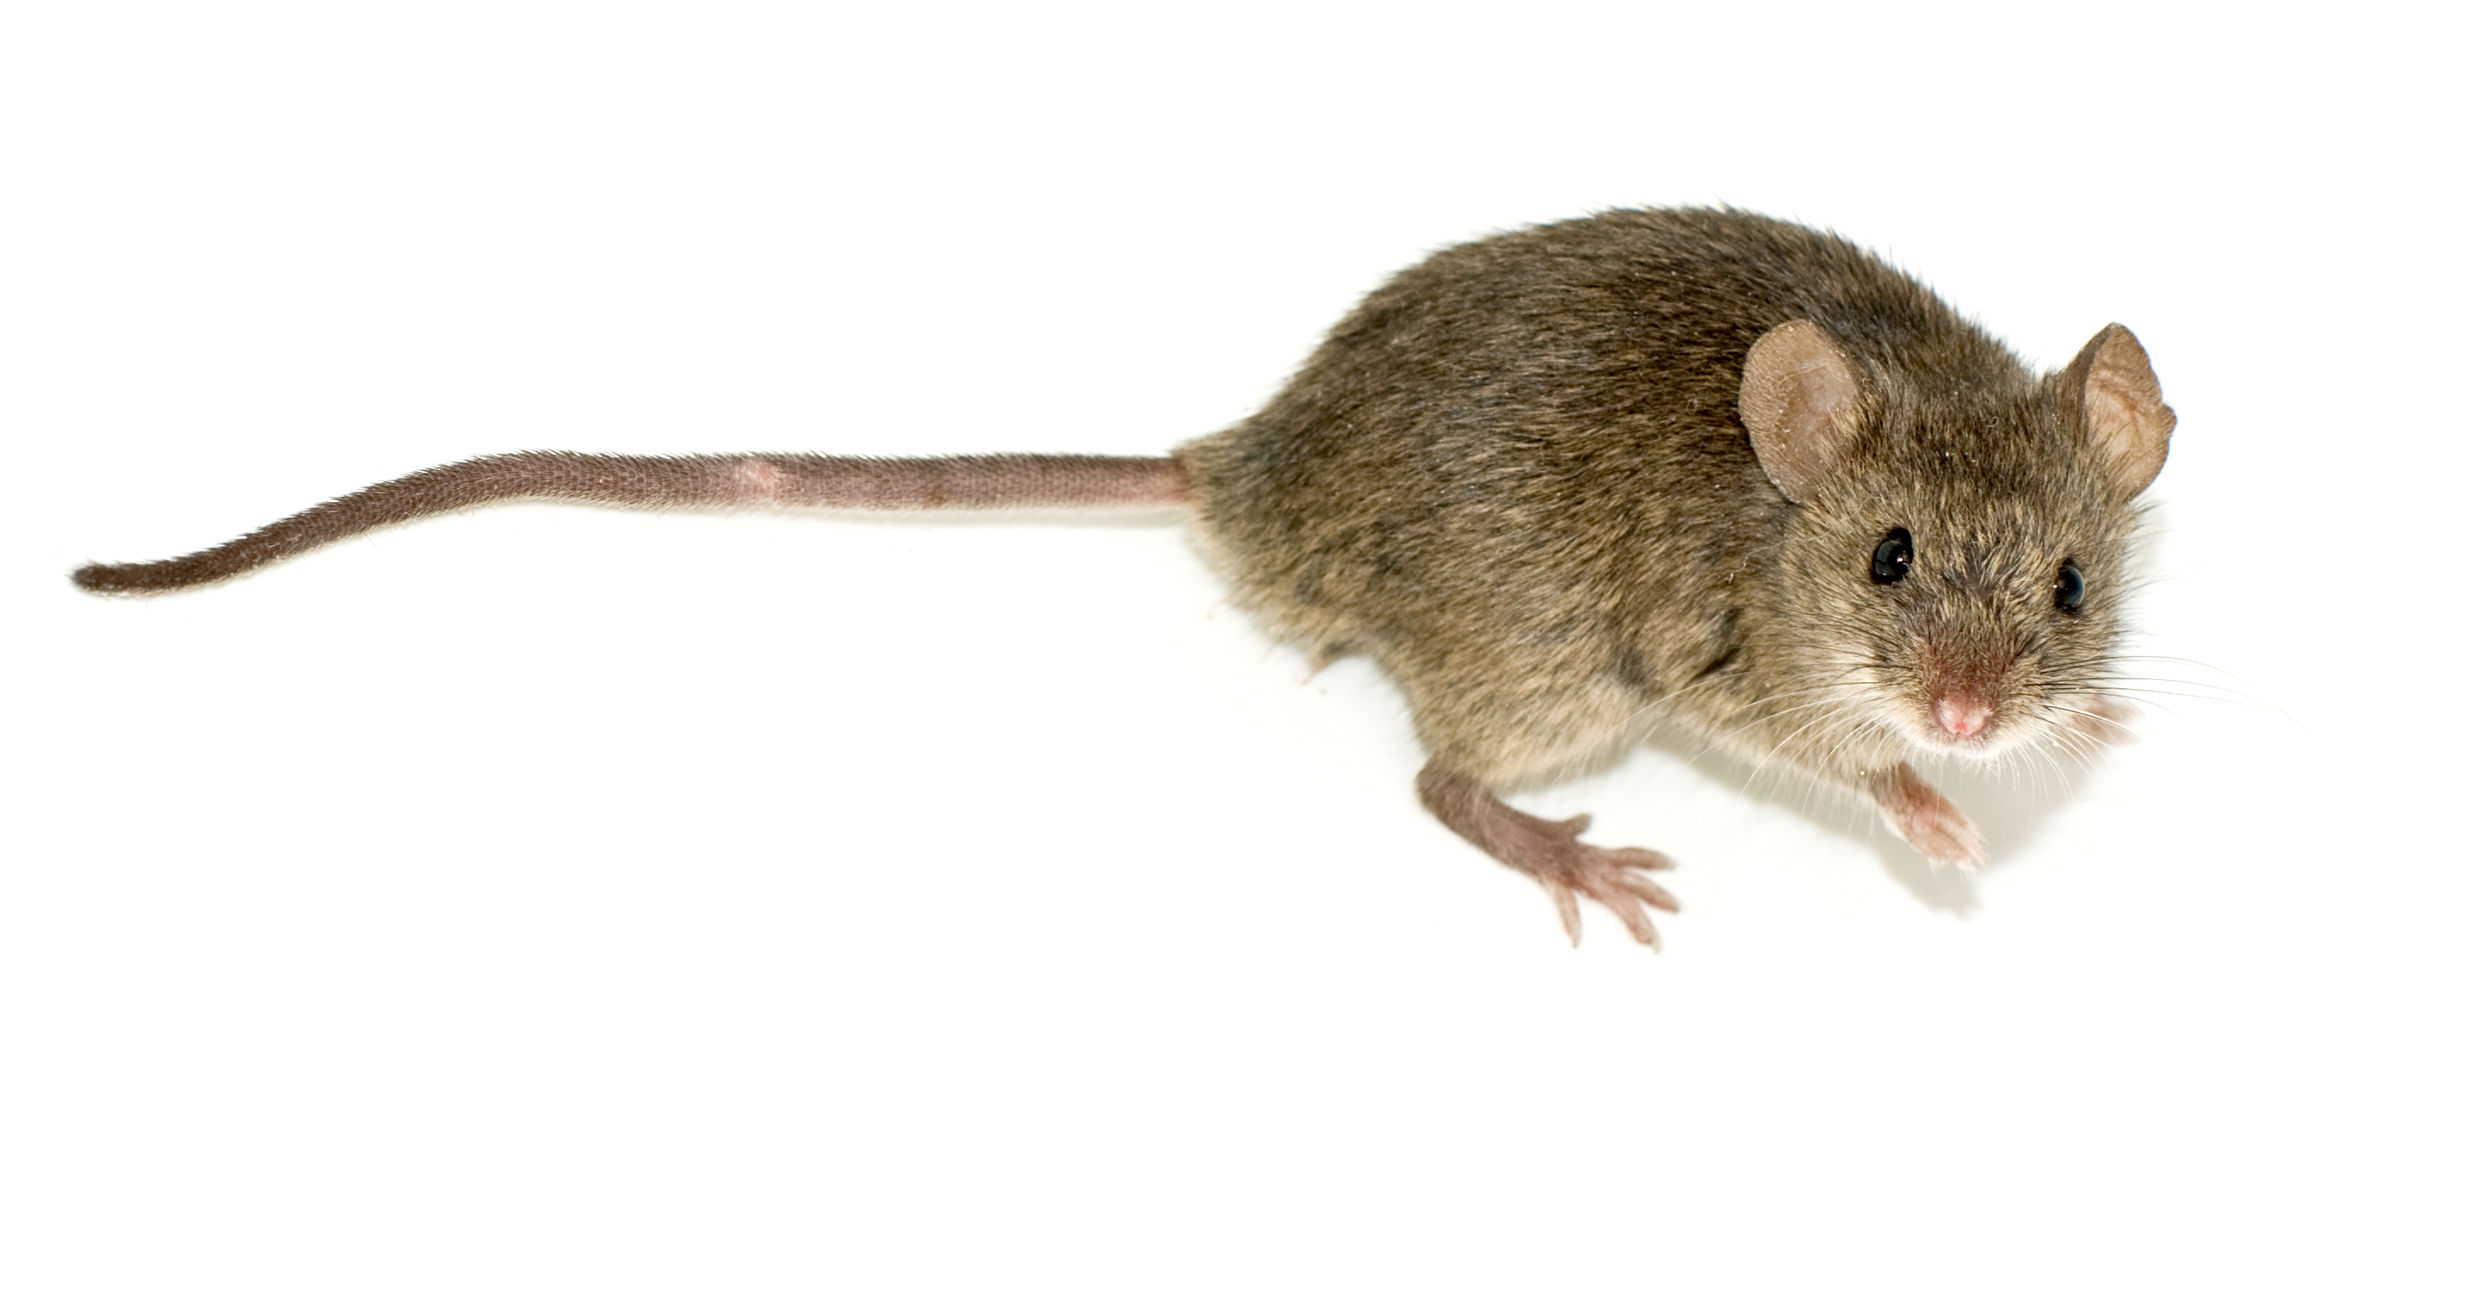
\includegraphics[width=1.0\textwidth]{static_images/mouse.jpg}
    \end{column}
\end{columns}


\end{frame}



%%%%%%%%%%%%%%%%%%%%%%%%%%%%%%%%%%%%%%%%%%%%%%%%%%%%%%%%%%%
%%%%%%%%%%%%%%%%%%%%%%%%%%%%%%%%%%%%%%%%%%%%%%%%%%%%%%%%%%%
%%%%%%%%%%%%%%%%%%%%%%%%%%%%%%%%%%%%%%%%%%%%%%%%%%%%%%%%%%%


\begin{frame}{Latent variable models: Astronomical catalogs}

\begin{columns}
    \begin{column}{0.5\textwidth}

The Sloan Digital Sky Survey systematically photographed the night sky
from the earth's surface.  Astronomers wish to create a catalog of stars
and galaxies and their properties that can be searched through and analyzed
statistically, e.g. for evidence of dark matter.
\citep{regier2019cataloging}

\vspace{1em}

Each individual image contains distortion from that particular night's
atmosphere and telescope configuration.  The shape and identity of the
astronomical objects are latent variables, and the distortion is common
to all astronomical objects in a particular image.  The typical shape
and variability of the distortion is common to all images.

    \end{column}
    \begin{column}{0.4\textwidth}
        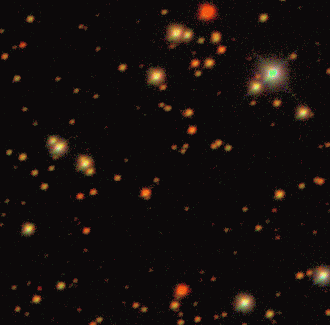
\includegraphics[width=1.0\textwidth]{static_images/sdss.png}
    \end{column}
\end{columns}


\end{frame}



%%%%%%%%%%%%%%%%%%%%%%%%%%%%%%%%%%%%%%%%%%%%%%%%%%%%%%%%%%%
%%%%%%%%%%%%%%%%%%%%%%%%%%%%%%%%%%%%%%%%%%%%%%%%%%%%%%%%%%%
%%%%%%%%%%%%%%%%%%%%%%%%%%%%%%%%%%%%%%%%%%%%%%%%%%%%%%%%%%%


\begin{frame}{Latent variable models}

    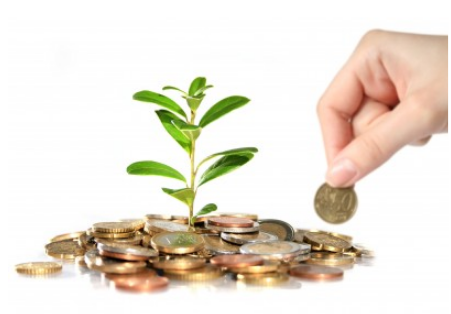
\includegraphics[width=0.3\textwidth]{static_images/microcredit.png}
    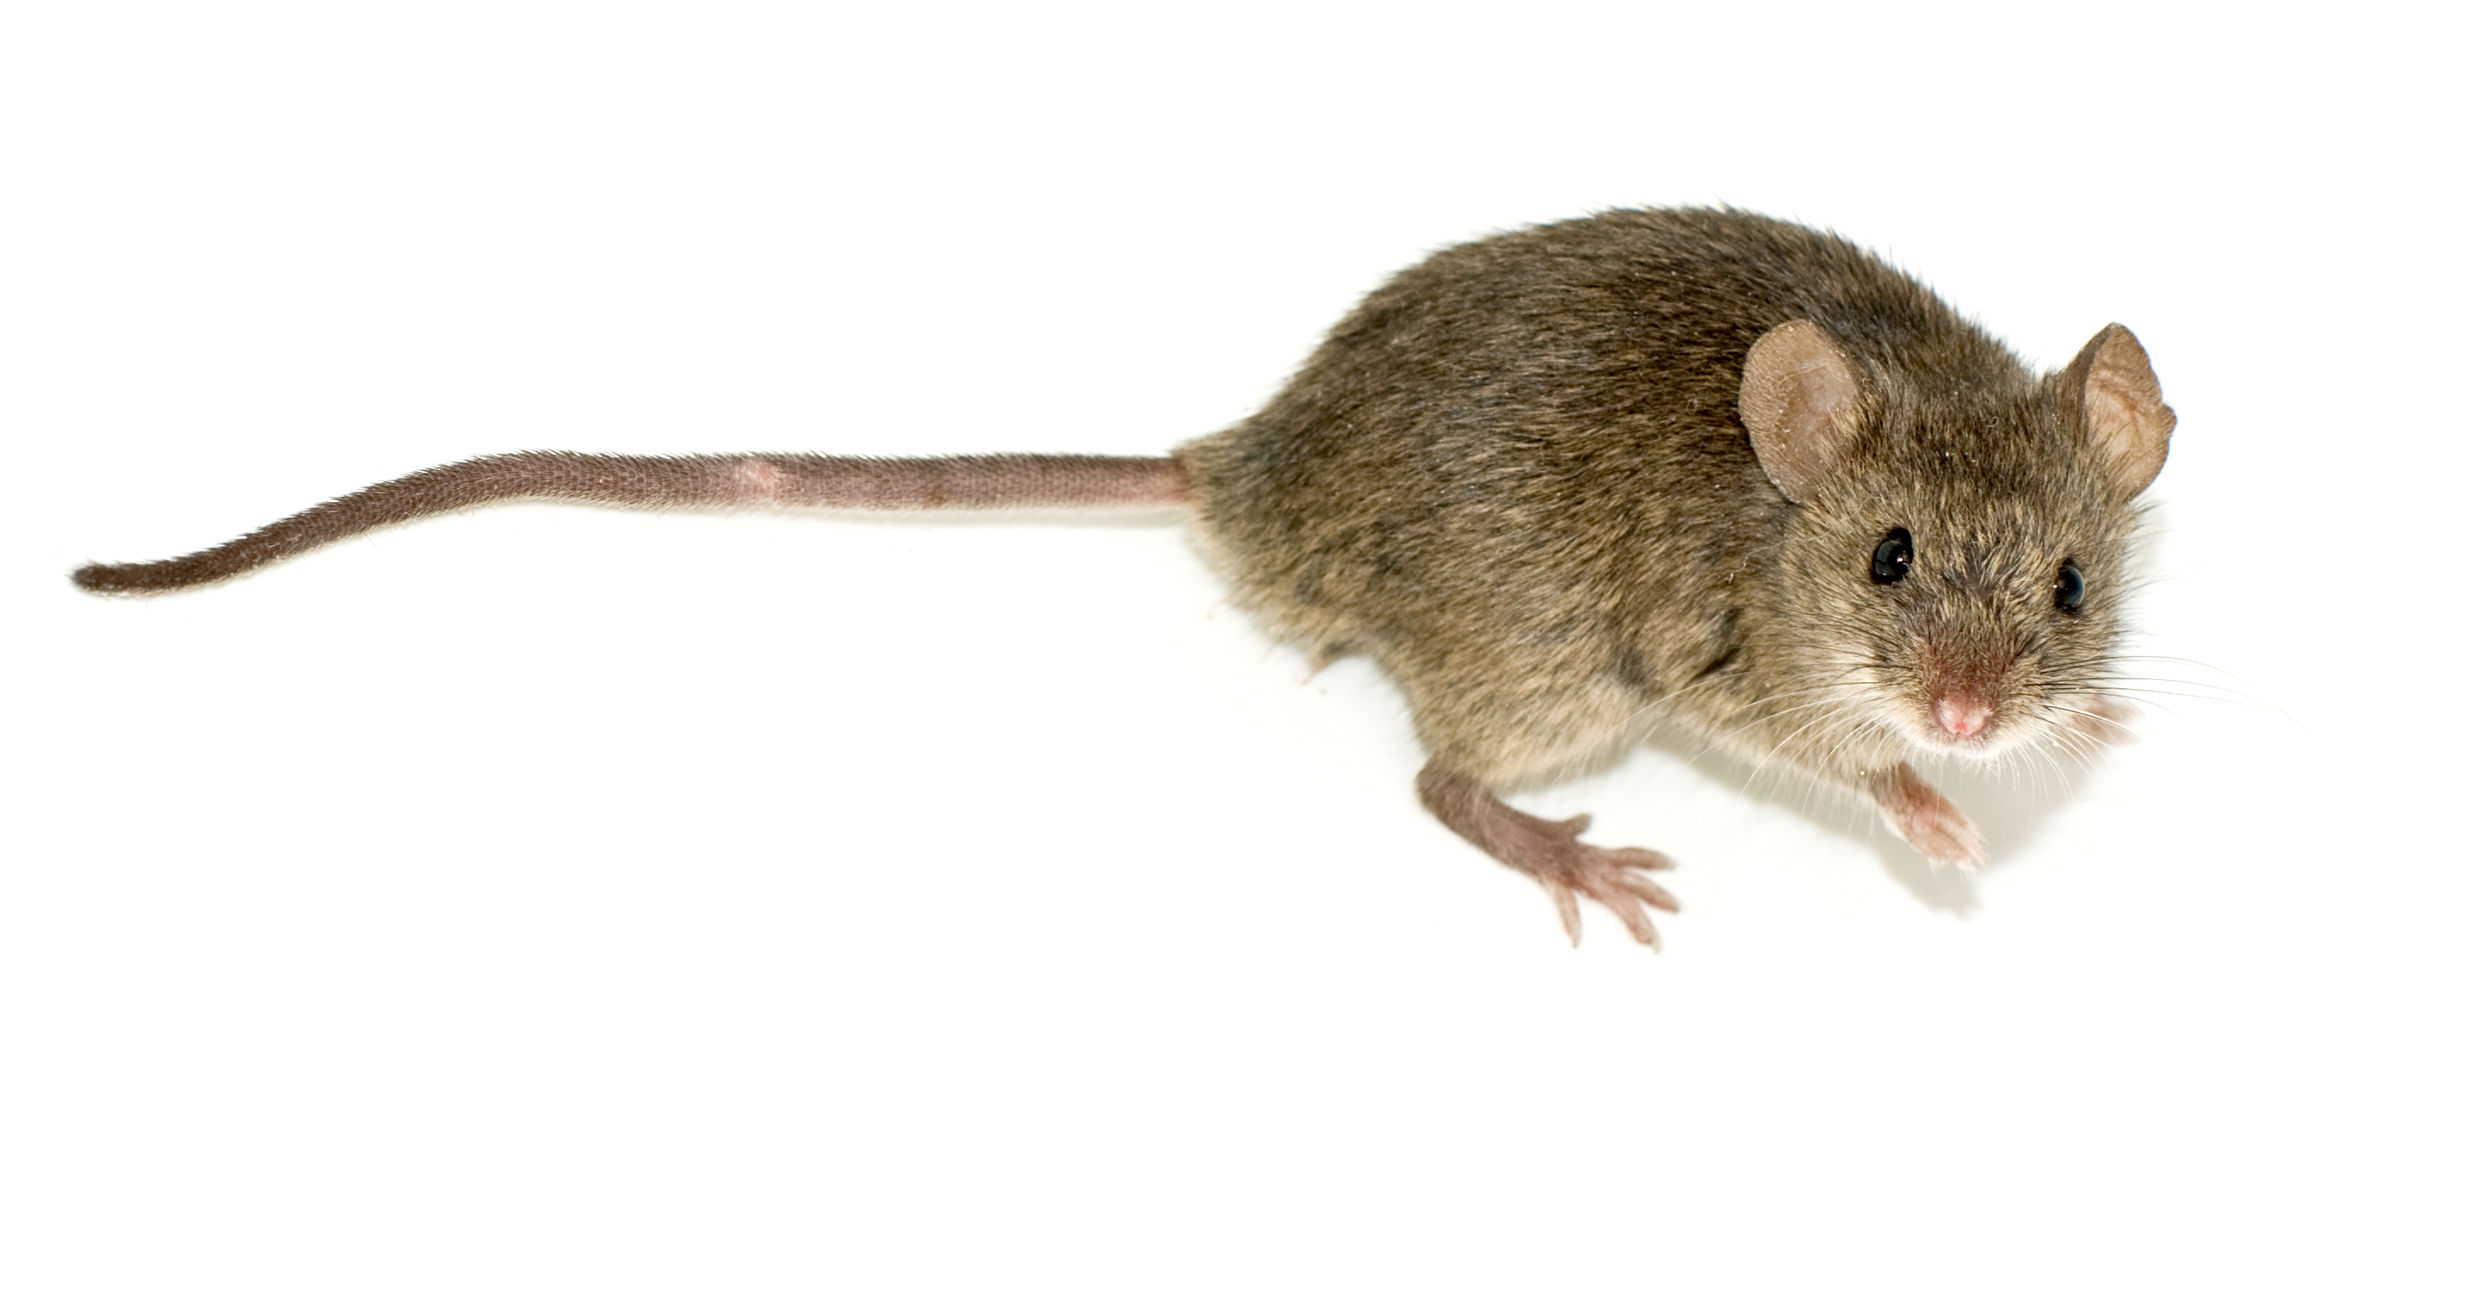
\includegraphics[width=0.3\textwidth]{static_images/mouse.jpg}
    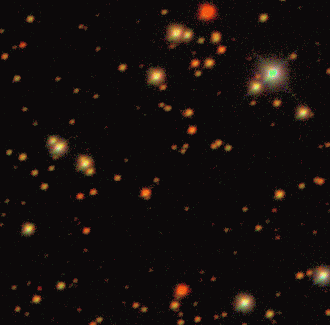
\includegraphics[width=0.3\textwidth]{static_images/sdss.png}

\vspace{3em}

Each of these models exhibits
\begin{itemize}
    \item High dimensional ``local'' latent structure
    \item Low-dimensional ``global'' parameters of primary interest
    \item Possibly complicated dependence between the two
        (knowledge of the local variables informs the value of the globals,
        and vice-versa)
\end{itemize}

\end{frame}
